
\section{Motivation}\label{sec:motivation}

In this section, we conduct a quantitative study  composed of several tests, in order
to deeply analyze the software tax that logging writes need to pay.
The setup of our testing platform is detailed in Section \ref{sec:eval}.

\iftrue
\vspace{1ex}
\noindent\framebox[\columnwidth][s]{
	\parbox{\dimexpr\linewidth-2\fboxsep-2\fboxrule}{$\vmathbb{O1}$. \em
		The  preallocation  strategy significantly
		boosts the performance of database logging writes.
}}
\vspace{0.5ex}
\else
\ul{$\vmathbb{O1}$. \em
	The  preallocation  strategy significantly
	boosts the performance of database logging writes.
}
\fi

Database logging depends on   persistent file writes.
In the first test, we study an SSD (Samsung PM1725a)  which has supercapacitor-enabled PLP   and features low write latency. 
We use Fio~\cite{1fioFlex42:online} to create a file and repeatedly append data until it reaches 1GB, 
with 4KB per   request, each followed by   {fdatasync}. 
We configure two file creation options in Fio.
One preallocates a 1GB file at   start.
The other begins with an empty file that  grows to 1GB gradually. 
The file system is Ext4.
This test aims to analyze the effect of  preallocation. 

\begin{figure}[!t]
	\centering
	\begin{subfigure}[t]{0.49\columnwidth}
		\centering
		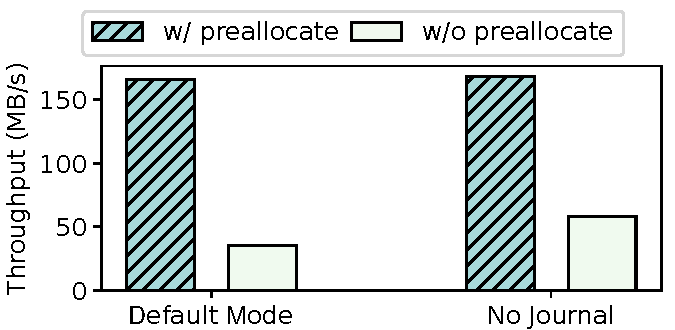
\includegraphics[width=\columnwidth, page=1]{./fig/mot/mot-preallocate.pdf}
		\caption{The Impact of Preallocation on File Writes.}
		\label{fig:Mot:mot-preallocate}
	\end{subfigure}
	\hfill
	\begin{subfigure}[t]{0.49\columnwidth}
		\centering
	 	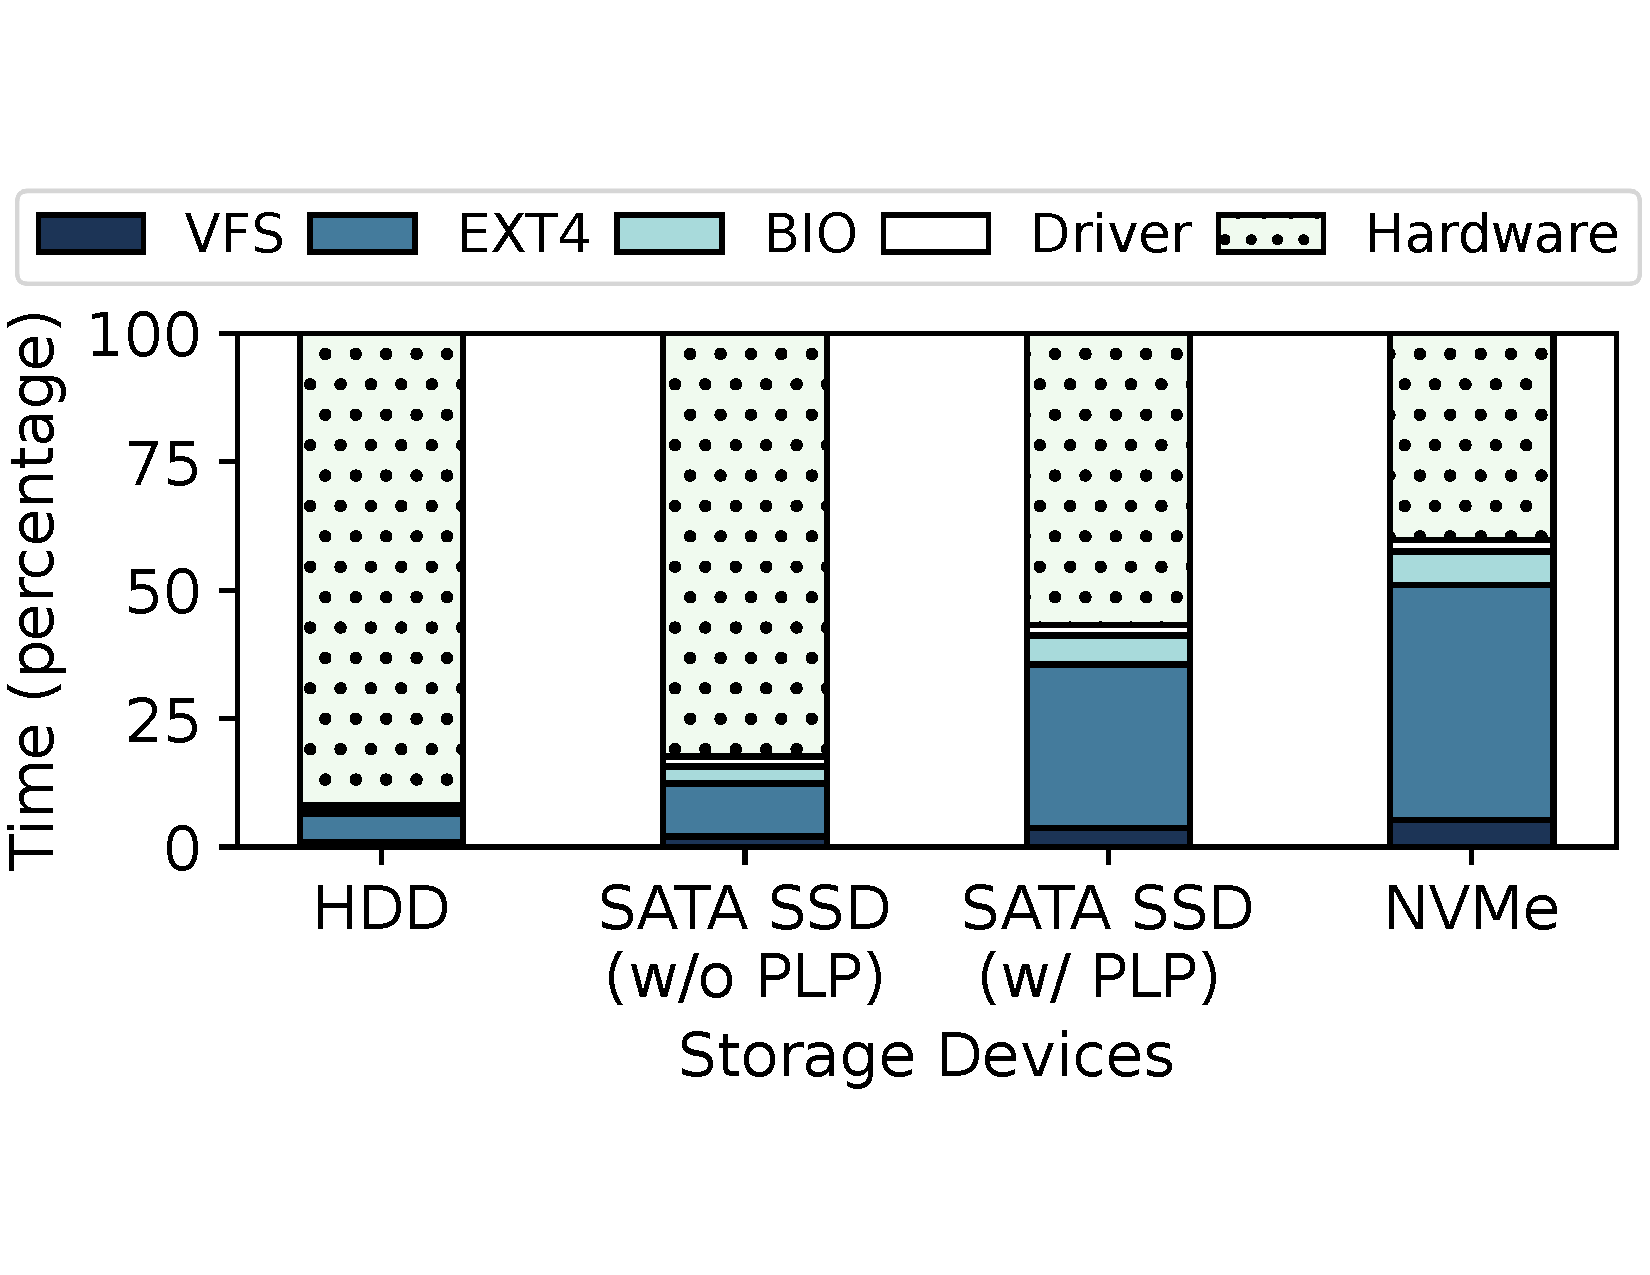
\includegraphics[width=0.8801\columnwidth, page=1]{fig/mot/mot-breakdown2.pdf} 
		\caption{The Breakdowns  on the File I/O Path.}
		\label{fig:Mot:workload-breakdown}
	\end{subfigure}
	\vspace{-0.5ex}
	\caption{The Impact of Preallocation on File Writes and the Breakdowns on the File I/O Path with Varying Devices.}
	\vspace{-2ex}
\end{figure}

\autoref{fig:Mot:mot-preallocate} shows the throughput (bandwidth in MB/s) 
for writing data to two files when Ext4 is mounted in two modes. 
In the default \texttt{data=ordered} mode,  
the   throughput increases from 35MB/s to 166MB/s.
This improvement occurs because preallocation eliminates on-demand block allocation 
and avoids metadata journaling.
Comparatively, for the growing file,
each appending write   triggers a cascade of  operations on the critical path, including the query of block groups for free space,
the modification of block bitmap upon allocation,  the update of file's extent tree, 
and the composition and commit of metadata changes to the journal.
These operations   construct a serious performance cost that becomes increasingly problematic with fast storage devices like the  SSD we are using.
Even if we disable   journaling, i.e., `No Journal' in \autoref{fig:Mot:mot-preallocate},
preallocation still yields   significant performance improvements. Additionally, 
preallocation is likely to ask Ext4 to assign contiguous blocks to a file,
which is
 beneficial for the sequential appending I/O pattern of database logging. 
To sum up,
 {\em we shall adopt the preallocation-like strategy 	to better exploit the	device- and OS-level optimizations
for accelerating   logging writes}.

\iftrue
\vspace{1ex}
\noindent\framebox[\columnwidth][s]{
\parbox{\dimexpr\linewidth-2\fboxsep-2\fboxrule}{$\vmathbb{O2}$. \em
The   software tax is dominated by file system operations  and badly
impairs the performance of database logging.}
}
\vspace{0.5ex}
\else
\ul{$\vmathbb{O2}$. \em
The runtime software tax is dominated by file system operations  and badly
impairs the performance of  logging.
}
\fi

We next assess the  software tax imposed per   write with a preallocated file.
We use four   devices for a comprehensive analysis:
a   hard disk (WDC WD20EZWX), a SATA SSD without PLP (Samsung 870EVO), a SATA SSD with PLP (Samsung PM893), and an  NVMe SSD with PLP (Samsung PM1725a). 
We measure  the time cost of each software layer   using Intel VTune Profiler \cite{GetStart56:online}. 
The I/O pattern is the same   as used in the first test with a preallocated file under Ext4 file system.
\autoref{fig:Mot:workload-breakdown} presents the breakdowns for hardware and software layers with four devices.
In spite of  preallocation, {\em the runtime
	software tax increasingly dominates   I/O latency
	as   devices become faster}, reaching  60.2\% for the   NVMe SSD. 

Specifically,
  Ext4
   is the predominant latency
source with the NVMe SSD, contributing about 46.3\%.
 Although no structural change occurs to the file,
  frequent metadata operations persist, mainly due to searching
  for target block numbers
   in the
per-file mappings \cite{SSD:BypassD:ASPLOS-2024}.
{\em Moving such search operations off the critical path shall effectively
reduce the overall software tax}.

\iftrue
\vspace{1ex}
\noindent\framebox[\columnwidth][s]{
\parbox{\dimexpr\linewidth-2\fboxsep-2\fboxrule}{$\vmathbb{O3}$. \em
For non-preallocated log files, logging writes still incur severe  overhead, which  can be mitigated through a preallocation-like strategy.}
}
\vspace{0.5ex}
\else
\ul{$\vmathbb{O3}$. \em
	For non-preallocated log files, logging writes incur severe  overhead, which  can be mitigated through a preallocation-like strategy.}
\fi

\begin{comment}
:
before accepting data for the target file,
Ext4 asks for new blocks from the block group(s), updates the file's extent trees, and commits these metadata changes into the
 journal  for crash consistency. 
\end{comment}

\begin{figure}[!t]
\centering
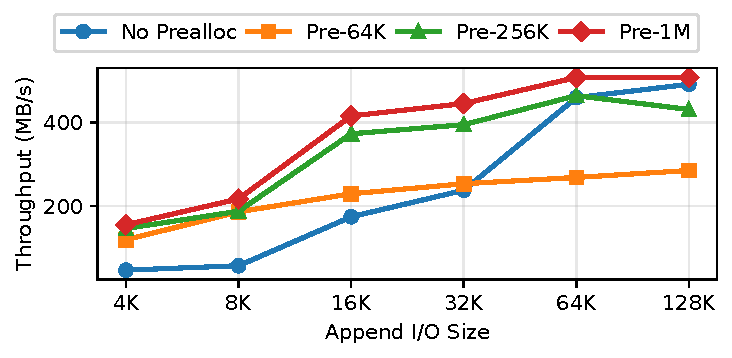
\includegraphics[width=0.9\columnwidth]{fig/mot/prealloc_throughput.pdf}
\vspace{-1ex}
\caption{The Impact of On-the-fly Preallocation on Appending Writes on a Dynamically Growing File.}
\label{fig:mot:prealloc-throughput}
\vspace{-4ex}
\end{figure}

Real-world databases may  use preallocated or growing log files,
 such as the binlog  of MySQL \cite{mysql2013mysql}.
As mentioned,
an appending write triggers costly runtime operations with   a growing file.
We investigate if there is a chance that we can accelerate file  writes issued to non-preallocated log files 
in a preallocation-like way.
In the third test, 
we append overall 10GB data to a file in the direct I/O mode
with the size per write being
4KB, 8KB, 16KB, 32KB, 64KB, and 128KB. They cover common database transaction sizes for logging
in practice.
We primarily create an empty file to complete this appending task.
The curve with dots in \autoref{fig:mot:prealloc-throughput} 
shows a rising throughput 
with the increase of I/O size. 
Next, we explicitly apply an on-the-fly  preallocation prior to each appending write. That is, we call fallocate to 
preallocate numerous blocks to the file
 before   appending data. Without loss of generality,
we extend the file in 64KB, 256KB, or 1MB at a time. We 
  initialize  preallocated blocks by filling zeros after      fallocate
to truly acquire the  space and invoke fsync to trigger journaling in advance.
By doing so, we intend to concretely prepare space  in a batched manner for one or multiple subsequent 
appending writes.

\begin{table}[!t]
	\centering
	{\large
		\renewcommand{\arraystretch}{1.3}%
		\caption{A Comparison between SOTA Designs.}
		\label{tab:mot:sota-comparison}
			\vspace{-1ex}
		\begin{adjustbox}{max width=0.5\textwidth}
			\begin{tabular}{lcccccc} 	
				\toprule
			Solutions	& \multicolumn{1}{c}{\makecell{No\\ hardware\\change}} 
				& \multicolumn{1}{c}{\makecell{Non-\\intrusive\\kernel}} 
				& \multicolumn{1}{c}{\makecell{Transparent\\support for\\applications}} 
				& \multicolumn{1}{c}{\makecell{Existing\\file system\\compatibility}} 
				& \multicolumn{1}{c}{\makecell{Compati- \\ bility  with  \\SATA SSD}} \\
				\midrule
				SPDK     & \checkmark & \checkmark & $\times$   & $\times$   & \checkmark  \\
				NVMeDirect & \checkmark & $\times$  & $\times$   & $\times$   & $\times$ \\
				Moneta-D   & $\times$   & $\times$  & \checkmark & \checkmark & \checkmark \\
				BypassD   & $\times$   & $\times$  & \checkmark & \checkmark & $\times$ \\
				\textcolor{blue}{\bf \odes} & \textcolor{blue}{\bf \Checkmark} & \textcolor{blue}{\bf \Checkmark} & \textcolor{blue}{\bf \Checkmark} & \textcolor{blue}{\bf \Checkmark} & \textcolor{blue}{\bf \Checkmark} \\
				\bottomrule
			\end{tabular}
		\end{adjustbox}
	}
	\vspace{-3ex}
\end{table}

In \autoref{fig:mot:prealloc-throughput},
the other 
three curves with squares, triangles, and diamonds represent the bandwidths
with dynamically preallocating 64KB, 256KB, and 1MB, respectively.
A comparison among four curves brings about two inspiring points.
First, {\em  on-the-fly preallocation, though incurring allocation and journaling overheads on the critical path, is likely to boost   write performance}.
For example, given the typical I/O size of 4KB, the throughput increases by 2.6$\times$, 3.2$\times$, and 3.4$\times$
with three spaces  allocated ahead, 
respectively. Note that 
preallocating a contiguous space causes file system  journaling once, whose cost
is much less than the accumulated cost of journaling for every small   write.
Secondly, {\em the effect of on-the-fly preallocation diminishes when the I/O size is close to or   greater
than the preallocation size}. A large I/O   itself will trigger   space allocation, and
preallocating space  turns to be neither necessary nor meaningful.

Furthermore, we have thought about what
we can do to improve beyond this test. 
Although {\em on-the-fly preallocation is effective when combining smaller writes with larger allocated space}, 
{\em Ext4 introduces substantial time cost for each allocation on the critical path} due to  space management and metadata journaling.
Our design must address this issue (see Section~\ref{sec:design}).

\begin{comment}
	Moreover,   uninitialized blocks shall be initialized 
	upon the factual write, 
	incurring additional cost.
\end{comment}

\begin{comment}

As shown in \autoref{fig:mot:prealloc-throughput}, the results reveal stark performance differences. For 4KB appends without preallocation (0K baseline), throughput is only 46.3 MB/s—each append triggers a jbd2 transaction for metadata updates. With 1MB step-wise preallocation, 4KB appends achieve 155.2 MB/s, a 3.4× improvement. This dramatic gain stems from amortizing jbd2 overhead: instead of journaling every 4KB append, metadata updates occur only every 1MB. However, larger append sizes show diminishing returns from preallocation. For 128KB appends, throughput improves modestly from 491.7 MB/s (baseline) to 508.1 MB/s (1MB prealloc)—only 3.4\% gain. This occurs because the relative cost of journaling per byte written decreases as append size increases. And the step-wise preallocation also introduces overhead on the critical path. Each \texttt{fallocate} call and subsequent initialization with zeros adds synchronous latency—for 1MB preallocation. While beneficial for small appends where jbd2 dominates, this overhead becomes proportionally significant for large appends where data movement already dominates. These findings motivate \odes's design optimizations: we employ asynchronous preallocation and initialization off the critical path, allowing small appends to benefit from reduced jbd2 overhead without penalizing large append performance.
\end{comment}

\iftrue
\vspace{1ex}
\noindent\framebox[\columnwidth][s]{
\parbox{\dimexpr\linewidth-2\fboxsep-2\fboxrule}{$\vmathbb{O4}$. \em
State-of-the-art solutions developed to reduce the software tax exhibit considerable limitations.}
}
\vspace{0.5ex}
\else 
\ul{$\vmathbb{O4}$. \em
	SOTA designs targeting the software tax have   limitations.}
\fi

Regarding the  evolution of storage devices,
researchers have studied the  software tax charged on file I/Os.
\autoref{tab:mot:sota-comparison} shows   state-of-the-art (SOTA) solutions in five dimensions. Intel
SPDK~\cite{SSD:SPDK:CloudCom-2017} and NVMeDirect  \cite{SSD:NVMeDirect:HotStorage-2016}  demand 
extensive reprogramming efforts  due to poor POSIX API compatibility, challenging the reliance of databases on standard file I/O interfaces.
Moneta-D \cite{SSD:Moneta-D:ASPLOS-2012} and BypassD~\cite{SSD:BypassD:ASPLOS-2024} are more compatible
with existing file systems and   databases. Nevertheless, they  require kernel changes and/or specialized hardware or 
software.
Take BypassD for illustration. It handles a request of mapping an in-file offset to  target block number through
a specialized IOMMU. Also, its implementation introduces more than 4,200 lines of code (LOC) in the Linux kernel.
  Furthermore, it only supports NVMe SSD.
 These
hinder its portability and usability. 
In all,
such drawbacks   limit the effectiveness of SOTA designs in general-purpose  production environments.

\begin{comment}
 

To address these challenges, we introduce \odes, an all-in-software solution that eliminates software tax for both preallocated and dynamically growing files. \odes decouples I/O operations from file management through eBPF-based interception and direct device access. For dynamically growing files, \odes employs an innovative donor-based allocation strategy using Ext4's \texttt{move\_extent} feature, enabling efficient block management without repeated journaling overhead. This approach preserves POSIX compatibility and access protection while facilitating seamless integration into existing database systems, remaining compatible with both SATA and NVMe SSDs.
\end{comment}